% Submission manuscript. Compile with pdfLaTeX (the Overleaf default).
\documentclass[12pt]{article}
\usepackage[a4paper,margin=1in]{geometry}
\usepackage[utf8]{inputenc}
\usepackage[T1]{fontenc}
\usepackage{amsmath}
\usepackage{newtxtext,newtxmath}
\usepackage{microtype}
\usepackage{graphicx}
\usepackage{booktabs}
\usepackage{makecell}
\usepackage{setspace}
\usepackage{newunicodechar}
\usepackage{xcolor}
\usepackage[hidelinks]{hyperref}

\graphicspath{{figures/}}

\newunicodechar{−}{\ensuremath{-}}
\newunicodechar{–}{--}
\newunicodechar{×}{\ensuremath{\times}}
\newunicodechar{≤}{\ensuremath{\leq}}
\newunicodechar{≈}{\ensuremath{\approx}}
\newunicodechar{±}{\ensuremath{\pm}}
\newunicodechar{∈}{\ensuremath{\in}}
\newunicodechar{→}{\ensuremath{\to}}
\newunicodechar{←}{\ensuremath{\leftarrow}}
\newunicodechar{·}{\ensuremath{\cdot}}
\newunicodechar{Σ}{\ensuremath{\Sigma}}
\newunicodechar{π}{\ensuremath{\pi}}
\newunicodechar{μ}{\ensuremath{\mu}}
\newunicodechar{ρ}{\ensuremath{\rho}}
\newunicodechar{τ}{\ensuremath{\tau}}
\newunicodechar{Δ}{\ensuremath{\Delta}}
\newunicodechar{ŷ}{\ensuremath{\hat{y}}}

\begin{document}

\begin{singlespace}
\begin{center}
{\Large\bfseries Supplementary material}\\[8pt]
{\large Separating mixing from selection: a leave-one-line-out\\[2pt]
benchmark and an audit protocol for cross-cell-line\\[2pt]
perturbation evaluation}\\[12pt]
{\normalsize Zhenghao Zhu$^{1}$, Di Cui$^{1,*}$}\\[4pt]
{\small $^{1}$Heze University, Heze, Shandong, China}\\[2pt]
{\small $^{*}$Correspondence: cuidi-nano@hotmail.com}
\end{center}
\end{singlespace}

\begin{singlespace}

\section*{Supplementary figure legend}

\noindent\textbf{Figure S1. Historical retrieval comparison against scGPT on matched targets.} The fine-tuned checkpoints are not part of the local snapshot, and every paired equal mix uses decoded H1 responses. (A) Per-target PDS for scGPT (scgpt\_r10) against equal mixing on the RPE1 holdout, over the 93 shared H1-panel targets. The recorded setup excludes RPE1 from fine-tuning. (B) The same comparison for scgpt\_check on K562. K562 is included in the recorded fine-tuning setup, so this is in-sample calibration, not a cross-line test. Dashed lines mark equality. Annotations give median PDS for scGPT and for equal mixing, the mean paired difference, and the win rate of equal mixing. (C) Mean paired difference in PDS against scGPT (95\% paired-bootstrap CI) for the target-agnostic mean response, equal mixing, and equal mixing plus centering on the 93 shared targets. RPE1 uses scgpt\_r10; K562 uses scgpt\_check and is in-sample.

\begin{center}
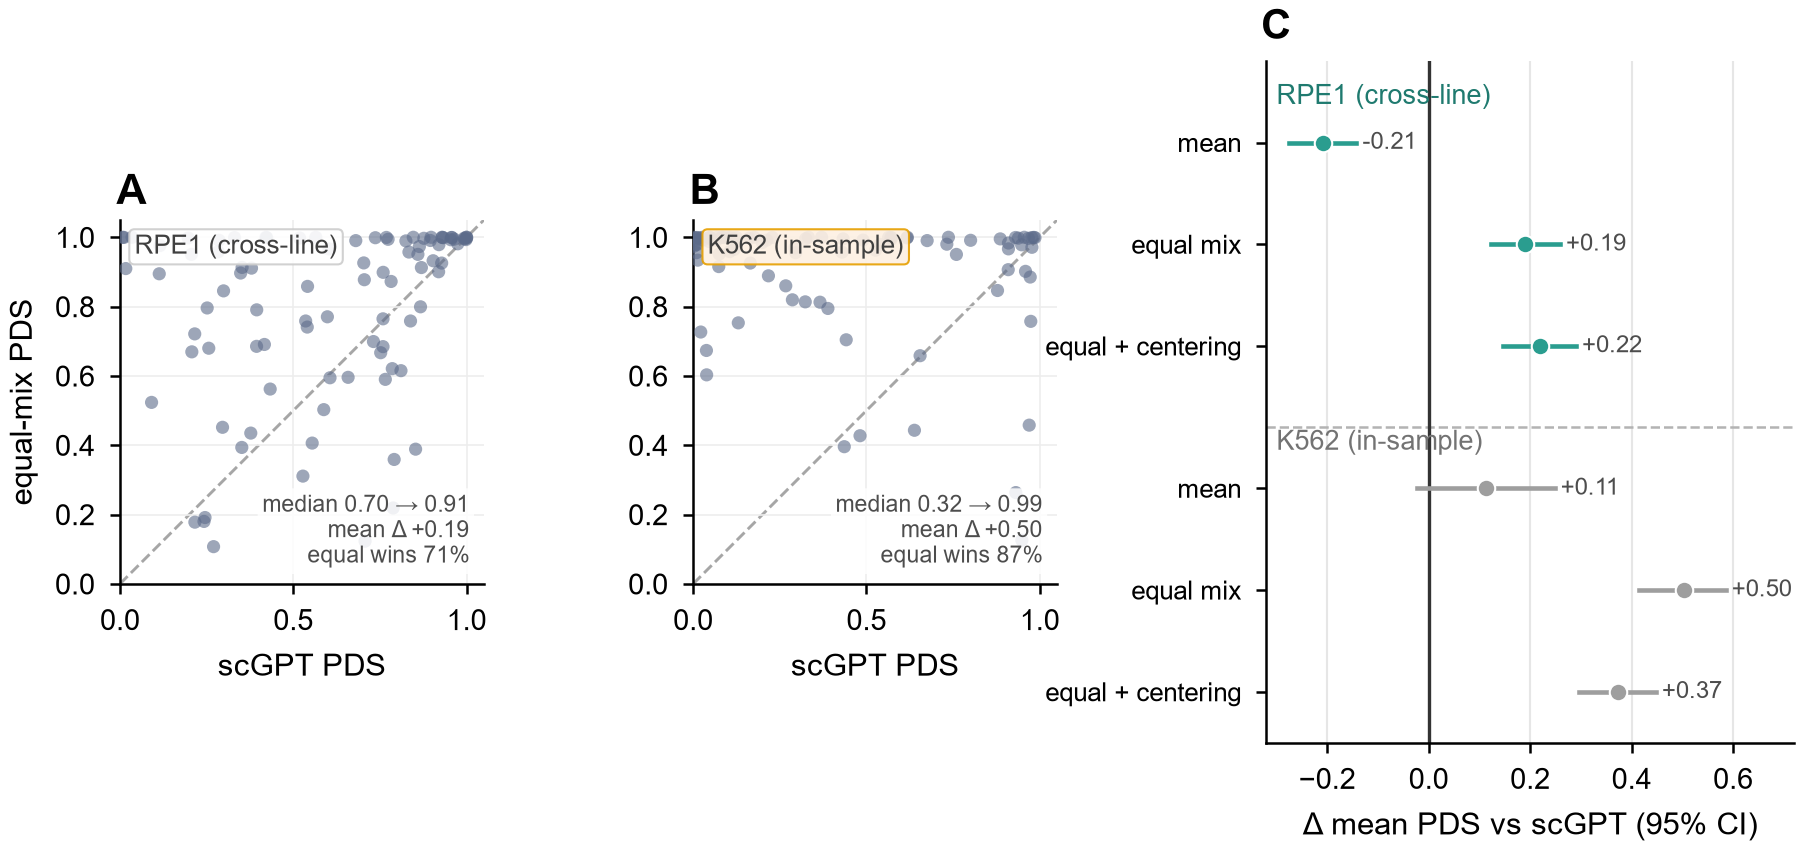
\includegraphics[width=\linewidth,height=0.68\textheight,keepaspectratio]{figS1_scgpt_baseline.png}
\end{center}


\clearpage
\section*{Table legends}

\noindent\textbf{Table S1. All methods, all holdouts.} Mean, median, paired difference versus equal mixing, 95\% bootstrap CI, Wilcoxon p, win rate, and median difference for every method and holdout.

\noindent\textbf{Table S2. Transfer determinants.} Per source–holdout pair: Spearman correlation between PDS and source response norm, and between PDS and self-log-fold-change, with p-values and pair sizes.

\noindent\textbf{Table S3. Variant scans.} Fixed-sample (1,000 queries per holdout) comparisons of centering variants and robust aggregation variants against equal mixing, with target-coordinate exclusion.

\noindent\textbf{Table S4. Historical scGPT baseline comparison.} Paired comparison of stored scGPT predictions against retrieval and mixing baselines on shared targets, for the RPE1 and K562 pools and both configurations. The recorded setup excludes RPE1 from fine-tuning and includes K562. RPE1 is the intended cross-line evaluation; K562 is in-sample calibration only. The fine-tuned checkpoints are not part of the local snapshot. Every paired equal-mix comparator uses decoded H1 responses. See Figure S1 and Supplementary Note 1.

\noindent\textbf{Table S5. Target-coordinate exclusion sensitivity.} (A) Equal-mixing median and mean PDS with and without target-coordinate exclusion for three Tier B holdouts. (B) Among queries whose target gene was in the evaluated positions, Spearman correlation between the per-query drop (PDS without exclusion minus PDS with exclusion) and the query's target-gene log fold-change, with bootstrap 95\% confidence intervals.

\noindent\textbf{Table S6. Gate decomposition.} Equal mixing on all targets versus the gate-selected subset, gated mixing on the gate subset, selection effect, mixing effect, Wilcoxon p-value, and win rate for each holdout.

\noindent\textbf{Table S7. Panel-wide exclusion sensitivity.} Main comparisons were recomputed with every target gene in the reference pool removed from both the ranked feature space and the denominator ($n-1$). This follows the cell-eval2 vcc2026 preset as closely as a full-pool benchmark allows. For each tier and holdout the table gives the number of positions removed and retained, equal-mixing mean and median PDS, and paired differences versus equal mixing for the mean response, raw mixing, mean centering, gated mixing (on the gate subset), and top-2 self-weighting, with 95\% bootstrap confidence intervals, Wilcoxon p-values, and win rates.

\noindent\textbf{Table S8. Supervised calibration.} Ridge, k-nearest-neighbor, and residual MLP mappings fitted on the held-out line's other stored response rows and evaluated by five-fold cross-validation. For each tier and holdout: mean (median) PDS, equal-mixing mean, paired mean difference with 95\% bootstrap confidence interval, Wilcoxon p-value, win rate, and median difference. This analysis uses held-out-line labels and is not a training-free transfer result. The target-coordinate-zeroed sensitivity and the target-label permutation are reported in Section 2.11. The permutation was applied within each training fold, after the fold split, so evaluation-target responses cannot enter training under another label. A second random seed was run for the residual MLP in the four holdouts where it had improved on equal mixing; the K562 and HCT116 gains reproduced and the HepG2 gain did not. P-values are nominal and not corrected; with thousands of paired targets, small differences can produce small p-values, so effect sizes and confidence intervals are the primary readout.

\noindent\textbf{Table S9. Source-side allocation.} For each Tier A holdout and each two-source state with a candidate line: actual gain of adding the candidate on the target line, pseudo gain measured on the existing sources, and the two leave-one-source-out components. Twelve decisions; Spearman and Pearson correlations are given in Section 2.13.

\noindent\textbf{Table S10. Calibration under no-exclusion scoring.} Mean PDS change versus equal mixing is given for $k$-means and random calibration at $k = 20, 50, 100$, and 200 in each Nadig line, with target-coordinate exclusion disabled. The exclusion-scored curves are in Fig. 7B for comparison.

\noindent\textbf{Table S11. Oracle and global rule-selection audit.} One tier, holdout, and candidate pool per row. The table gives candidate and target counts, equal-mix mean PDS, and per-target oracle mean. It names the best fixed rule and gives its mean. The descriptive heterogeneity gap is oracle minus best fixed, with a 95\% query-bootstrap interval. The permutation reference and excess over its mean accompany it. Split-half columns give the mean and gain for one global rule. Global rule-selection optimism is best fixed minus split-half. The oracle gap is oracle minus split-half. Oracle gain over equal mixing is also reported. Gate rows give apparent gain, composition, and within-subset gain. They have no oracle heterogeneity gap. Tahoe rows audit eight calibration-budget rules using per-condition $\Delta$PDS against zero. The permutation reference is descriptive. The oracle gap does not estimate selection bias. The audit compares a per-target oracle with one global rule.

\noindent\textbf{Table S12. Source-response coherence summaries.} For each holdout the table gives the number of queries on the diagnostic subset. It also gives mean pairwise, mean minimum pairwise, and mean centered pairwise cosine of the unit-normalized source responses, the mean log$_{10}$ response norm across sources, and mean equal-mix PDS on the same targets. Raw and centered associations use Spearman correlation. The log-norm-partial column uses the standard rank-residual procedure described in Methods. The mix-truth cosine and its association with PDS use held-out responses. Source coherence uses source rows on the full stored axis; H1 responses are decoded estimates. These associations are within-panel summaries.

\noindent\textbf{Table S13. Tahoe drug-panel coherence and retrieval summaries.} Seven lines, 648 shared active conditions. The table reports pairwise, minimum pairwise, and centered pairwise cosine of the six unit-normalized source responses, plus the mean resultant. It gives the mean cosine between the six-source equal mix and the held-out response, raw and centered. It gives the mean truth--truth cosine of the candidate pool, and the mean, 95th, and 99th percentiles of mix-to-other-condition cosine. The competitor-tail column is derived from PDS. Scores use the tie midrank and read the true score from the matching reference-matrix entry, so PDS is bounded at 1. The alignment-controlled column uses the standard rank-residual procedure. Alignment and pool summaries use held-out responses and cannot serve as source-only diagnostics. These entries are within-panel summaries.

\noindent\textbf{Table S14. GEARS baseline.} For each Tier A holdout: number of matched queries, best early-stopping epoch, GEARS and equal-mixing mean (median) PDS, paired mean and median differences with 95\% bootstrap confidence intervals, Wilcoxon p-values, win rates, and the paired comparison against the target-agnostic mean response. Scoring uses the equal-mixing pool, target-coordinate exclusion, and denominator, and every Tier A query has a prediction. GEARS was trained leave-one-line-out on unit-normalized responses; its zero cell-graph input is an additive decoder term, so this is equivalent to the absolute-expression form (Methods), with one hyperparameter configuration per fold and no hyperparameter search. The mean-response column locates GEARS between the two training-free baselines.

\noindent\textbf{Table S15. GEARS multi-seed reproducibility.} Three random seeds per Tier A holdout. For each seed the table gives the best early-stopping epoch, GEARS mean PDS, the paired mean and median differences versus equal mixing, and the win rate. Summary columns give the seed average and the seed-to-seed standard deviation of the mean difference. They also give the fraction of targets where GEARS scored below equal mixing under all three seeds, the Pearson and Spearman correlation of per-target PDS between seeds, and the median and 90th percentile of the per-target standard deviation across seeds. Hyperparameters were identical across seeds. Only initialization and training randomness changed. Source data are in \texttt{outputs/seed\_runs/multiseed\_summary.csv} and the merged per-seed result files.

\noindent\textbf{Table S16. Pool-free metrics for the equal mix and GEARS.} Per-query cosine similarity, Pearson correlation, top-50 Jaccard overlap, and relative mean squared error before and after a per-query scalar calibration, with the target coordinate zeroed in both prediction and truth. (A) Mean values for equal mixing, centered mixing, the mean response, gated mixing, and GEARS in each Tier A fold, over all queries and over the gate-selected subset. (B) Paired differences with 95\% bootstrap confidence intervals, Wilcoxon p-values, and win rates for equal mixing against GEARS, the mean response, and centered mixing, and for equal mixing against gated mixing on the gate subset. PDS recomputed from the rebuilt predictions matches the stored benchmark values exactly. Source data are in \texttt{outputs/secondary\_metrics\_A.csv} and \texttt{outputs/secondary\_metrics\_A\_pairs.csv}.

\noindent\textbf{Table S17. Twelve-line Tahoe panel.} For each of the twelve lines, on the 646 conditions shared by all lines: equal-mix mean and median PDS with eleven sources, unique-top fraction, mean PDS with other doses of the same drug excluded, mean single-source PDS, and, for the seven original lines, the same equal-mix mean with six sources on the same 646 conditions; mean pairwise and minimum pairwise cosine of the eleven unit-normalized source responses and their within-line Spearman correlation with per-condition PDS; and the fraction of full-pool score resamples below the descriptive threshold at $k=50$ and $\tau=0.92$. The five added lines are SW480, NCI-H460, SNU-423, A-172, and KATO III; the two dropped conditions are the 0.05 $\mu$M doses of 4EGI-1 and 9-ING-41. Source data are in \texttt{outputs/tahoe12\_full.csv}, \texttt{outputs/p7\_646\_full.csv}, \texttt{outputs/tahoe12\_coherence.csv}, and \texttt{outputs/tahoe12\_pilot.csv}.

\noindent\textbf{Table S18. Calibration in the twelve-line Tahoe panel.} Mean PDS change versus equal mixing for k-means and random calibration at $k=20$, 50, 100, and 200. Original 95\% row-pooled bootstrap confidence intervals are given for the fixed twelve-line panel mean and each line separately. Unique-condition intervals and existing-split sensitivity envelopes are reported in Table S20. Each line was split three times into 161 evaluation and 485 calibration conditions, with the same PCA-ridge map and selection rules as the seven-line panel. Source data are in \texttt{outputs/tahoe12\_deltas.csv} and \texttt{outputs/tahoe12\_ci.csv}.

\clearpage

\noindent\textbf{Table S19. Genuinely small Nadig reference pools.} Each draw selects distinct targets from the balanced 638-target panel. The selected targets are both queries and competitors. Predictions use the other three lines and stay fixed across draws. There are 5,000 draws per size at seed 0. Entries show the mean across draws and the 2.5th--97.5th percentiles of subset means in brackets. These percentiles are not confidence intervals. Crossing is the percentage of draws whose mean reaches the post-hoc 0.92 threshold. Exclusion removes each query's target coordinate from the prediction and every candidate, with separate renormalization. The no-exclusion columns retain it. Source data are in \texttt{outputs/pilot\_small\_pool.csv}; that file also reports the balanced full-pool baseline and unique-top fractions.

\vspace{6pt}
{\scriptsize
\setlength{\tabcolsep}{3pt}
\renewcommand{\arraystretch}{1.1}
\begin{tabular}{@{}lrcrcr@{}}
\toprule
Held-out & $m$ & \makecell{Exclusion mean\\{[subset quantiles]}} & \makecell{Crossing\\(\%)} & \makecell{No-exclusion mean\\{[subset quantiles]}} & \makecell{Crossing\\(\%)} \\
\midrule
K562 & 50 & 0.811748 [0.757600, 0.864800] & 0.00 & 0.847713 [0.795200, 0.897200] & 0.16 \\
K562 & 100 & 0.809630 [0.772397, 0.847102] & 0.00 & 0.845976 [0.811500, 0.880800] & 0.00 \\
RPE1 & 50 & 0.834816 [0.771600, 0.900000] & 0.40 & 0.861993 [0.800400, 0.922400] & 2.94 \\
RPE1 & 100 & 0.833770 [0.790097, 0.878000] & 0.00 & 0.861274 [0.820097, 0.902400] & 0.26 \\
HepG2 & 50 & 0.796190 [0.738800, 0.854000] & 0.00 & 0.831428 [0.775200, 0.885610] & 0.04 \\
HepG2 & 100 & 0.794275 [0.755200, 0.833000] & 0.00 & 0.829675 [0.792400, 0.866703] & 0.00 \\
Jurkat & 50 & 0.813080 [0.757600, 0.867610] & 0.00 & 0.846113 [0.792790, 0.896010] & 0.20 \\
Jurkat & 100 & 0.811205 [0.772498, 0.849600] & 0.00 & 0.844369 [0.807700, 0.880402] & 0.00 \\
\bottomrule
\end{tabular}
}

\clearpage

\noindent\textbf{Table S20. Drug calibration interval sensitivity.} Panel means give equal weight to the fixed observed lines. Repeated condition scores are averaged within split, then equally over available splits. Unique-condition intervals use 10,000 bootstrap draws at seed 0. Shared condition weights preserve cross-line pairing on observed supports. The split-CI envelope takes the smallest lower and largest upper endpoint across three existing splits. Each split uses two-sided $\alpha = 0.05/3$. Adjustment is within each row across splits only. The envelope is a conservative sensitivity range over existing fits. Neither interval resplits or retrains, and neither estimates uncertainty across new lines. The twelve-line random-selection envelope at $k = 200$ spans zero. Seven-line source data are in \texttt{outputs/tahoe\_calibration\_ci\_sensitivity.csv}; twelve-line source data are in \texttt{outputs/tahoe12/tahoe12\_ci\_sensitivity.csv}. These files also retain the original row-pooled estimates and per-line results.

\vspace{6pt}
{\scriptsize
\setlength{\tabcolsep}{3pt}
\renewcommand{\arraystretch}{1.1}
\begin{tabular}{@{}rrlrcc@{}}
\toprule
Lines & $k$ & Selection & \makecell{Unique-condition\\mean $\Delta$PDS} & \makecell{Unique-condition\\95\% interval} & \makecell{Split-CI\\envelope} \\
\midrule
7 & 20 & k-means & $-$0.032594 & [$-$0.036323, $-$0.028962] & [$-$0.043043, $-$0.024308] \\
7 & 20 & random & $-$0.043785 & [$-$0.047169, $-$0.040529] & [$-$0.050109, $-$0.037367] \\
7 & 50 & k-means & $-$0.013570 & [$-$0.016270, $-$0.010883] & [$-$0.018058, $-$0.007675] \\
7 & 50 & random & $-$0.019335 & [$-$0.022300, $-$0.016433] & [$-$0.024286, $-$0.013014] \\
7 & 100 & k-means & $-$0.008806 & [$-$0.011345, $-$0.006249] & [$-$0.012877, $-$0.002873] \\
7 & 100 & random & $-$0.011969 & [$-$0.014787, $-$0.009107] & [$-$0.016977, $-$0.006070] \\
7 & 200 & k-means & $-$0.006498 & [$-$0.009098, $-$0.003893] & [$-$0.011685, $-$0.001177] \\
7 & 200 & random & $-$0.008049 & [$-$0.010899, $-$0.005300] & [$-$0.013409, $-$0.002249] \\
\midrule
12 & 20 & k-means & $-$0.047089 & [$-$0.051837, $-$0.042675] & [$-$0.057763, $-$0.038905] \\
12 & 20 & random & $-$0.044924 & [$-$0.048733, $-$0.041298] & [$-$0.054581, $-$0.037631] \\
12 & 50 & k-means & $-$0.020096 & [$-$0.022944, $-$0.017342] & [$-$0.027556, $-$0.013704] \\
12 & 50 & random & $-$0.019689 & [$-$0.022304, $-$0.017214] & [$-$0.026952, $-$0.013443] \\
12 & 100 & k-means & $-$0.010223 & [$-$0.012257, $-$0.008313] & [$-$0.015119, $-$0.005836] \\
12 & 100 & random & $-$0.009854 & [$-$0.011734, $-$0.008054] & [$-$0.014522, $-$0.006063] \\
12 & 200 & k-means & $-$0.004606 & [$-$0.006285, $-$0.002864] & [$-$0.008189, $-$0.000489] \\
12 & 200 & random & $-$0.004017 & [$-$0.005442, $-$0.002574] & [$-$0.007069, +0.000408] \\
\bottomrule
\end{tabular}
}

\clearpage

\noindent\textbf{Table S21. Metric positive and negative controls.} For 300 uniformly sampled queries per holdout: mean and median PDS, 95\% bootstrap interval, fraction above 0.5, fraction at or above 0.9, and mean cosine to the truth. Predictions are the true response, equal mixing, the target-agnostic mean, a mismatched response, gene-shuffled truth, sign-flipped truth, and truth plus matched-norm Gaussian noise at 0.25, 0.5, 1, 2, and 4 times the response norm. All reference rows stayed in the pool. Scoring used target-coordinate exclusion, per-reference renormalization, and tie midranks. Source data are in \texttt{outputs/metric\_controls.csv}.

\noindent\textbf{Table S22. Candidate-pool composition control.} Balanced 638-query Nadig panel. Pools of 50 and 100 rows each contain the true response. Compositions are random, hard, easy, coherent, incoherent, strong, and quiet, with the full-pool level for comparison. Candidate selection uses source responses only. Equal mixing, centered mixing, single-source, and mean-response predictions are scored on identical pools under target-coordinate exclusion. Random pools were repeated 200 times. Source data are in \texttt{outputs/pool\_composition\_control.csv} and \texttt{outputs/pool\_composition\_rankings.csv}.

\clearpage
\section*{Supplementary Notes}

\subsection*{Supplementary Note 1. scGPT fine-tuning configuration and checkpoint provenance}

The following is the recorded fine-tuning configuration. The fine-tuned weights and complete run records are not part of the local snapshot. Both runs were specified to start from the released scGPT\_human weights (Cui et al. [10]). The pretrained encoder, value encoder, and transformer encoder were loaded from \texttt{best\_model.pt}; the expression decoder was trained from scratch. Fine-tuning used the K562 GWPS essential screen (Replogle et al. [1]), with 8,323 of 8,563 gene symbols present in the scGPT vocabulary. Counts were converted to log1p(CPM). Each target contributed at most 80 cells, and all 10,691 non-targeting cells were used as controls. The first run selected 143,984 cells per epoch (2,999 batches at batch size 48) and covered 1,836 target labels. The pseudobulk run required at least 20 cells per target, which kept 1,806 targets and 143,596 cells per epoch. The sampling seed was 42.

A training batch contained 48 cells and 1,536 genes drawn at random, with every target position in the batch forced into the gene subset. Perturbation cells received a flag with a one at the target gene; control cells had an all-zero flag. Perturbation cells were paired with a randomly drawn control cell as input, so the flag carried the target identity. Optimization used Adam at 10$^{-4}$ with a step decay of 0.9 per epoch, dropout 0.2, gradient clipping at 1.0, mixed precision, and two epochs. Both checkpoints used this optimization schedule.

scgpt\_check used cell-level targets. The decoder output plus the input expression was fitted to the measured log1p(CPM) of the perturbed cell over all positions. The epoch-1 weights were used for scoring. scgpt\_r10 used pseudobulk targets. For each target, the response was $d = \log_2((\text{mean CPM perturbed} + \epsilon)/(\text{mean CPM control} + \epsilon))$ over genes with control CPM at least 1, clipped to ±4. The cross-target weighted mean was subtracted, and the decoder's final layer was initialized to the identity (coefficient 1, bias 0, with 0.002-scale noise). The target gene's position stayed in the loss with a weight of 2,000 that decayed linearly to 1 over the first 1,000 batches, and genes with $|d| > 0.1$ received a fivefold weight. The epoch-2 checkpoint was scored. Its prediction was the decoder output minus the control input, and the cross-target mean was added back on the 18,080-gene axis before scoring (7,753 of 18,080 genes matched).

The recorded prediction setup used 1,000 control cells per context. Stored predictions were scored by \texttt{scripts/bench\_scgpt\_baseline.py} with the same pool, target-coordinate exclusion, and denominator as the retrieval baselines. Training is implemented in \texttt{scripts/scgpt\_ft\_gwps.py}; the mean correction is \texttt{scripts/add\_pb\_mean.py}. Expected checkpoint locations were \texttt{outputs/scgpt\_ft} (scgpt\_check, \texttt{model\_ep1.pt}) and \texttt{outputs/scgpt\_ft\_r10} (scgpt\_r10, \texttt{model\_ep2.pt}). Neither fine-tuned checkpoint is part of the local snapshot; the pretrained weights are a separate model. RPE1 is excluded from the recorded fine-tuning setup. K562 is in-sample for both configurations and is reported only as a calibration for scgpt\_check. Every paired equal-mix comparator includes a decoded H1 response. The stored scoring summaries describe this configuration.

\noindent\textbf{Evaluation.} Stored predictions cover the 93 H1-panel targets whose symbols map to the scGPT vocabulary. RPE1 is the intended cross-line evaluation. K562 is in-sample calibration only. Predicted deltas were stored on the 18,080-gene axis and restricted to the evaluation positions. They use the same pool, exclusion, and denominator as the mixing baselines, paired on the 93 common targets (88 for the gated comparison). Every paired equal mix uses decoded H1 responses.

\subsection*{Supplementary Note 2. Audit checklist}

Each item is a yes/no check. The listed scripts produce the relevant output. A checked item means the output exists and is reported. It does not certify the choice. The same checklist is in \texttt{AUDIT\_CHECKLIST.md} in the released repository.

\begin{itemize}
\item[$\circ$] \textbf{Equal-mix baseline.} Report the training-free matched-source mix and the target-agnostic mean on the same targets. \texttt{scripts/bench\_transfer\_nadig.py}, \texttt{scripts/bench\_transfer.py}, \texttt{scripts/audit\_numbers.py}.
\item[$\circ$] \textbf{Composition versus selection.} Report the oracle, the best fixed rule, the split-half estimate, and the draw count. Score gated and equal mixing on shared targets. \texttt{scripts/selection\_audit.py}, \texttt{scripts/selection\_figure.py}.
\item[$\circ$] \textbf{Centering.} Validate it per dataset and line pair. Do not apply it by default. \texttt{scripts/selection\_audit.py}, \texttt{scripts/make\_tables.py}.
\item[$\circ$] \textbf{Scoring policy.} Name target-coordinate exclusion and tie handling. Report paired intervals and one alternative policy. \texttt{scripts/bench\_scope\_sensitivity.py}, \texttt{scripts/secondary\_metrics.py}, \texttt{scripts/bench\_transfer\_analysis.py}.
\item[$\circ$] \textbf{Retrieval baseline.} Give any learned model the same targets, pool, and scoring policy. \texttt{scripts/bench\_transfer.py}, \texttt{scripts/bench\_transfer\_nadig.py}, \texttt{scripts/bench\_scgpt\_baseline.py}, \texttt{scripts/gears\_baseline.py}.
\item[$\circ$] \textbf{Small calibration set.} Compare selected labels with random labels and with the uncalibrated mix. Report both exchange routes. \texttt{scripts/phase1\_budget\_curve.py}, \texttt{scripts/phase1\_selection\_pilot.py}, \texttt{scripts/phase2\_source\_budget.py}, \texttt{scripts/phase2\_exchange\_summary.py}.
\item[$\circ$] \textbf{Pool-specific level.} Resample the realized pool. State any stopping threshold as post hoc. \texttt{scripts/regime\_summary.py}, \texttt{scripts/tahoe\_cal\_ci.py --sensitivity}, \texttt{scripts/pool\_composition\_control.py}.
\item[$\circ$] \textbf{Coherence.} Report within-panel rank summaries with partial controls. Do not treat them as a measurement rule. \texttt{scripts/tahoe\_coherence.py}, \texttt{scripts/tahoe\_coherence\_fast.py}, \texttt{scripts/regime\_diagnostic.py}, \texttt{scripts/tahoe\_partial\_check.py}.
\end{itemize}

\end{singlespace}

\end{document}
